\subsection{DroNet: Learning to Fly by Driving}

In their paper, Loquercio \etal~\cite{dronet}~propose a ResNet with only 8
layers, with an average accuracy only 1\% below ResNet-50 for the same
regression task. The objective function is, in fact, a combination of two
regressions allowing a drone to navigate in urban environments. Their network,
as seen in Fig.~\ref{fig:dronetoriginal}, contains two fully connected
layers: one for the steering commands of the drone, one for the collision
detection probability.

\begin{figure}[h]
	\center
	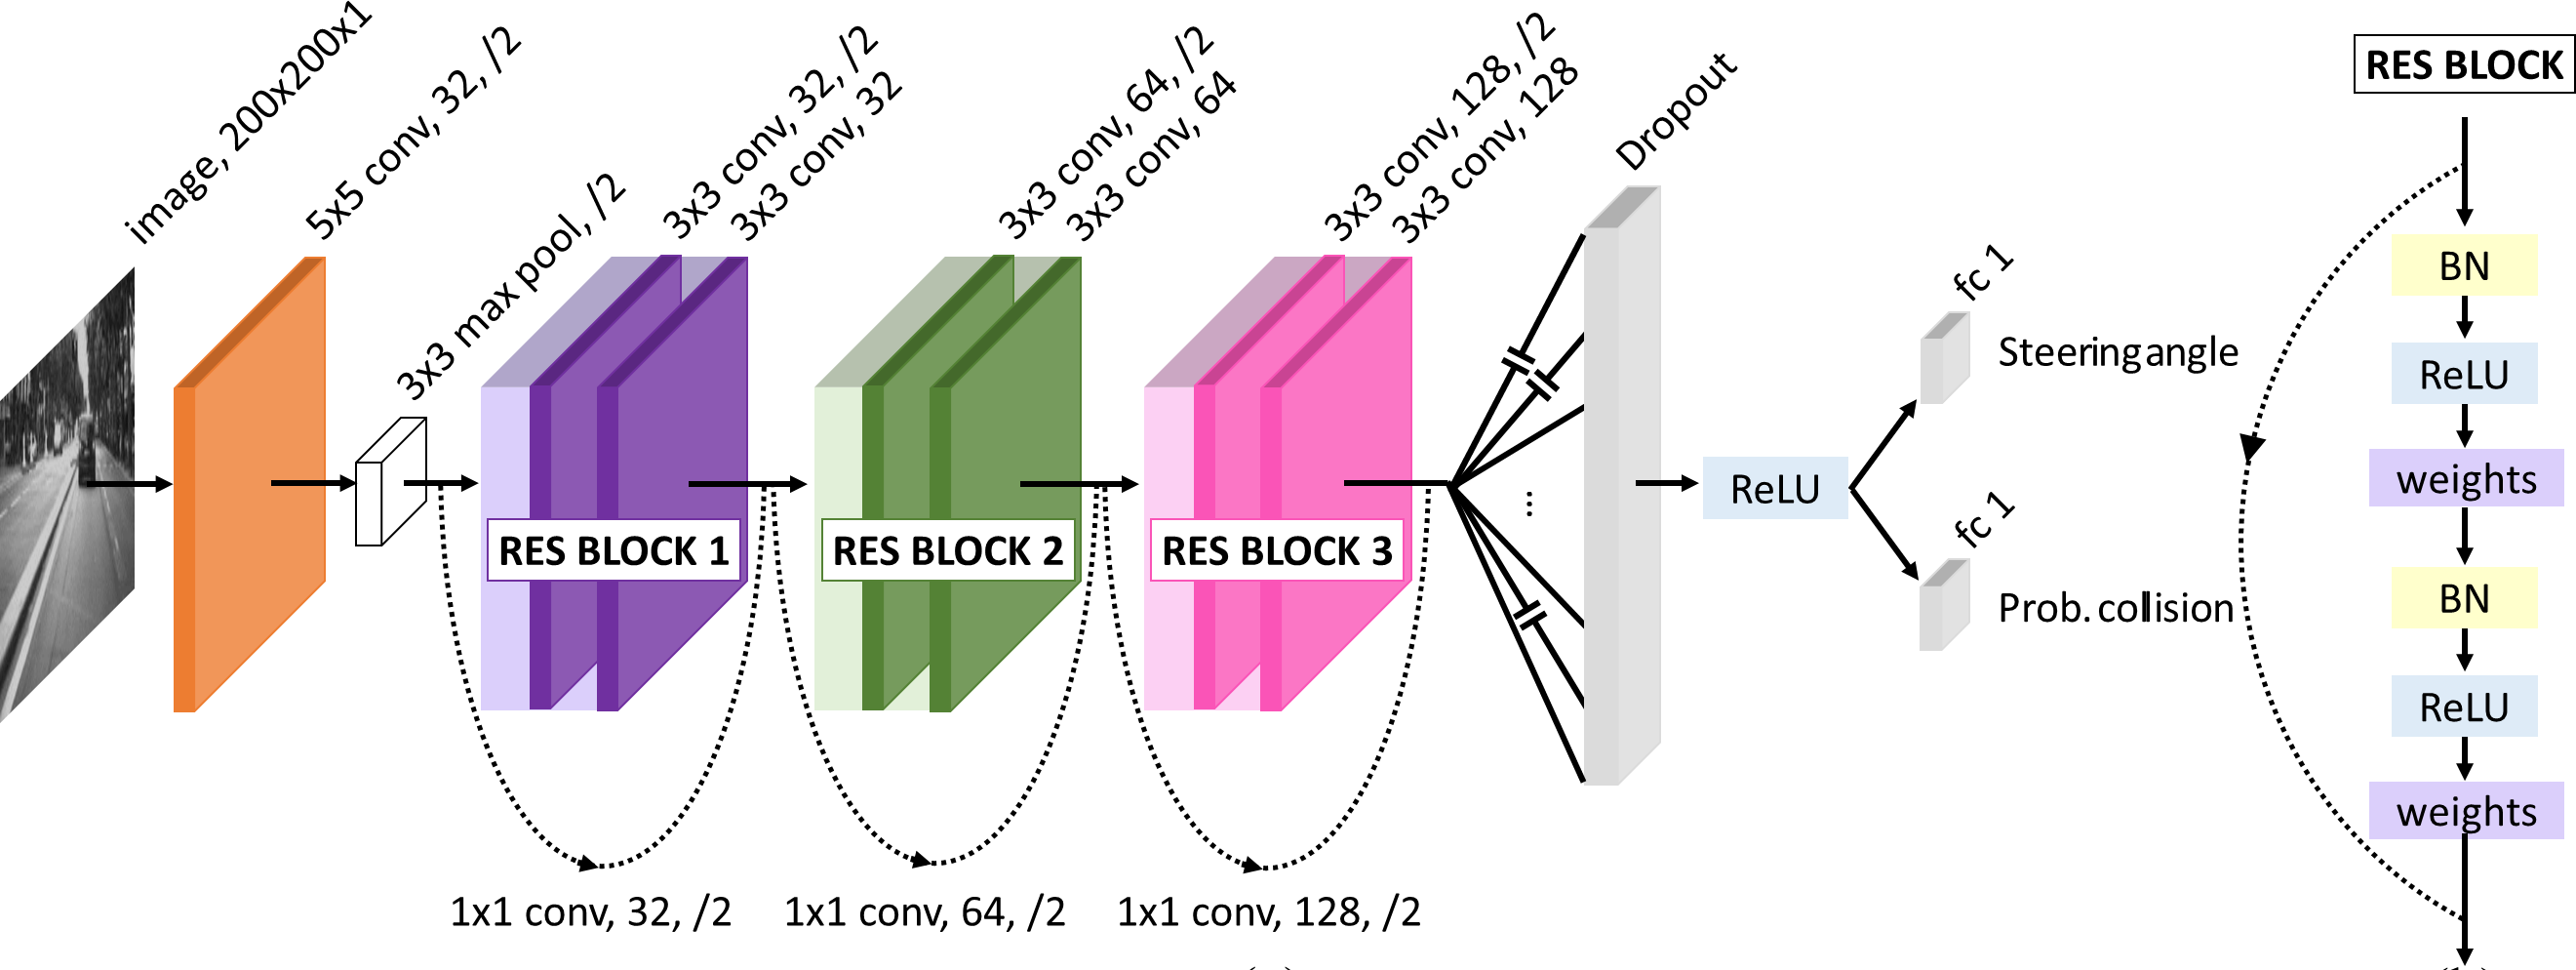
\includegraphics[width=\textwidth]{figure/dronet.png}
	\caption{Original DroNet model~\cite{dronet}.}
	\label{fig:dronetoriginal}
\end{figure}

What makes this model an attractive choice is its impressive performance when
compared to ResNet-50, with only $81\times$ fewer parameters, thus making it
well suited for embedded applications such as drone racing.\\

The network was trained on an outdoor dataset of $70,000$ car driving images
from Udacity's project, as well as a custom bicycle dataset of $32,000$
pictures they have collected for the collision detection. As for the input
specifications, the format used is a $200\times200$ grayscale center crop of
the original image, annotated with steering angles and binary collision labels.

\subsubsection{Modifications} \label{section:dronet-mods}

In order to use this model for detecting the center of a racing gate, its fully
connected layers had to be removed and replaced with one of size $N$
corresponding to the number of region proposal windows, as explained on
page~\pageref{fig:regionproposal}. 

The softmax activation function~\ref{equ:softmax} is used for this last layer,
since it transforms the activations of each output neuron into a probability,
where the sum of each output probability equals to one. It is defined as:

\begin{equation}
	\label{equ:softmax}
	f(\mathbf{s})_i=\frac{e^{s_i}}{\sum_j^C e^{s_j}},
\end{equation}

where $C$ corresponds to the number of classes ($N+1$ windows in this
instance), $\mathbf{s}$ are the prediction scores inferred by the network, and
$s_i$ is the evaluated prediction probability.\\

As for the loss function, it is the categorical cross-entropy, also referred to
as softmax loss, and is defined as:

\begin{equation}
	\label{equ:catcrossentr}
	CE=\displaystyle-\sum_i^C t_i log(f(s)_i)
\end{equation}

with $t_i$ being the ground truth for class $i$: either 0 or 1, since $t$ is a
one-hot encoded vector.\\

% Help from here: https://gombru.github.io/2018/05/23/cross_entropy_loss/

Furthermore, the input layer has been adapted to be used for this application,
by resizing it to $255\times340\times C$, corresponding to $255$ rows of the
input tensor for the image height, $340$ for the columns of the tensor and the
image with, and lastly $C$ channels to be set whether a grayscale or an RGB
input image is used.\\

Apart from those topography-related modifications, the parameters used for
training, such as the optimizer and the learning rate, were left identical: the
Adam optimizer is used with its default hyperparameters. Additional
modifications are brought to the fully-connected layers during the experiments,
which are explained in the corresponding chapter.

